% 紧致性
% 覆盖|子覆盖|紧子集|拓扑空间|紧邻域|紧空间|分离性

\pentry{连续映射和同胚\upref{Topo1}}

有的时候,研究包含了无穷多个点的子集会涉及到很多并不是那么重要的性质和细节.有些子集的行为,看起来就像是一个点或者几个点,把它揉成一个或几个点也无关紧要,有一点类似于等价类划分把等价元素都揉成了同一个.可以被这样揉成少数几个点的子集,是用以下定义的“覆盖”来描述的.

\subsection{覆盖}

给定任何集合$X$和它的一个子集$A$,我们常常可以用一系列$X$的子集$X_i$来把$A$包括在这些子集的并集里,这种行为叫做\textbf{用$\{X_i\}$来覆盖$A$}.比如说,取集合$\mathbb{R}$,那么我们可以用一系列子集$\{[n, n+10)\}$来覆盖$\mathbb{R}$本身,其中$n$取遍所有整数.当然,覆盖的方式不止一种.

\begin{definition}{覆盖}
给定集合$A\subset X$.如果$X$的若干子集的集合$\{X_i\}\subseteq 2^X$满足$A\subseteq\bigcup X_i$,那么我们说集合$\{X_i\}$\textbf{覆盖}了$A$.称$\{X_i\}$为$A$的一个\textbf{覆盖(cover)}.
\end{definition}

当然,用$\{[n, n+10)\}$来覆盖$\mathbb{R}$有些浪费,我们只需要其中的一部分就足够覆盖$\mathbb{R}$了,比如说只取$n$是偶数,甚至只取$n$是$98$的倍数的情况.由此我们可以引出\textbf{子覆盖}的概念.

\begin{definition}{子覆盖}
给定集合$A\subseteq X$和它的一个覆盖$\{X_i\}$.如果$\{X_i\}$的某个子集$\{Y_i\}$也能覆盖$A$,那么显然$\{Y_i\}$也是$A$的一个覆盖,称它为\textbf{$A对于\{X_i\}$的子覆盖}.
\end{definition}

在拓扑学中,我们常常关心拓扑空间中开子集的性质.因为根据子拓扑的\autoref{Topol_def3}~\upref{Topol}以及开集的有限交封闭性,开子集构成的拓扑空间中的开集,都是原空间中的开集.因此我们会特别关注用开子集来进行覆盖.

\begin{definition}{开覆盖}
给定拓扑空间$X$和它的一个子集$A$.如果$A$有一个覆盖$\{X_i\}$.如果各$X_i$是开集,那么我们称这个覆盖为\textbf{$A$的开覆盖(open cover)}.
\end{definition}

\subsection{紧子集}

\begin{definition}{紧子集}\label{Topo2_def1}
给定拓扑空间$X$和它的一个子集$A$.如果不论取$A$的哪一个开覆盖$\{X_i\}$,总存在一个子覆盖$\{Y_i\}\subseteq \{X_i\}$,那么称$A$是$X$的一个\textbf{紧子集(compact subset)},或者说$A$在$X$中是\textbf{紧致(compact)}的,简称$A$是\textbf{紧}的.
\end{definition}

紧集就像若干点一样,任意开覆盖都有有限子覆盖.为了直观感受紧致性,我们可以考察通常的度量空间$\mathbb{R}$.开区间$(0,1)$不是紧致的,因为如果取覆盖是$\{(1/n, 1)\}$,那么这个覆盖的任何有限子集都不足以覆盖$(0, 1)$.但是,闭区间$[0,1]$是紧致的,像$\{(1/n, 1)\}$这样的族\footnote{族(family)是指集合的集合,见词条\upref{Set}.}是没法覆盖闭区间的.事实上,在$\mathbb{R}$中只有闭集是紧的,但直接证明非常麻烦,但使用\textbf{分离性}\upref{Topo5}中的方法就可以方便地证明.

一般来说,讨论拓扑空间$X$中的子集$A$是不是紧致的,直接从$X$中找一切可能的开覆盖很麻烦,但是用拓扑基就可以大大简化开覆盖的种类.这就引出了如下定理:

\begin{theorem}{}\label{Topo2_the1}
给定拓扑空间$X$和它的一个子集$A$,任取$X$的一个拓扑基$\mathcal{B}$.$A$是紧子集,当且仅当从$\mathcal{B}$得到的开覆盖都有有限子覆盖.
\end{theorem}

这个定理非常直白,因为$X$的开集都是$\mathcal{B}$的元素取并得到的.有了这个定理,我们可以把一个开覆盖中的每个开集再拆分成更小的开集的并.还是用$\mathbb{R}$度量空间举例:

\begin{example}{}\label{Topo2_ex1}
$\mathbb{R}$有一个拓扑基$\mathcal{B}=\{(a,b):a,b\in \mathbb{R}\}$,也就是说,$\mathcal{B}$是全体开区间的集合.对于集合$(0,1)$,我们可以取开覆盖$\{(-1,1/3)\cup(2/3,2), (1/4, 3/4)\}$,这个开覆盖中包含了两个开集.但是这个覆盖也可以看成是三个开区间构成的集合:$\{(-1,1/3), (2/3,2), (1/4, 3/4)\}$,而这三个开区间都来自$\mathcal{B}$.

\end{example}

如果拓扑空间$X$是自己的紧子集,那么我们说这个空间是一个\textbf{紧空间}.紧空间中的闭集,都是紧的,如同以下定理所说.

\begin{theorem}{}\label{Topo2_the2}
紧空间的闭子集都是紧的.
\end{theorem}

假设$X$是一个紧拓扑空间,而$A\subseteq X$是$X$的一个闭子集.假设$\{X_i\}_{i\in \mathbb{Z}^+}$\footnote{下角标表示$i$的取值范围是正整数}是$A$的一个开覆盖,而因为$A$是闭集,故$X-A$是开集.记$X_0=X-A$,那么$X_0\cup\{X_i\}_{i\in \mathbb{Z}^+}=\{X_i\}_{i=0, 1, 2, \cdots}$就是$X$的一个开覆盖.因为$X$本身是紧的,所以$\{X_i\}_{i=0, 1, 2, \cdots}$必然有有限子覆盖$\{Y_i\}$,其中$Y_i$只有有限多个,每个$Y_i$都是某个$X_j$.那么$\{Y_i\}$就是$A$的有限开覆盖.当然了,我们希望证明的是$\{X_i\}_{i\in \mathbb{Z}^+}$有有限子覆盖,只需要把$X_0$从$\{Y_i\}$中剔除,那么剩下的就是$A$的有限开覆盖,并且还是$\{X_i\}_{i\in \mathbb{Z}^+}$的子覆盖.

\subsection{局部紧}

有的时候,一个空间往往整体上不是紧的,但它总在部分看起来“好像”有紧性.这就像地球表面是弯曲的,但我们局部看来它很接近一个不弯曲的平面.为了说清楚什么叫做“部分”看起来是紧的,我们需要扩充一下邻域的概念:

\begin{definition}{紧邻域}
给定拓扑空间$X$和$x\in X$.如果存在紧子集$A\subseteq X$使得$x$是$A$的内点,那么称$A$是$x$的一个紧邻域.
\end{definition}

紧邻域不一定是开集,因此不一定是邻域.与之类似的概念还有“闭领域”,其含义也是以$x$作为内点的闭集.注意,不管是邻域、紧邻域还是闭邻域,它们的共性在于,$x$必须是它们的内点,也就是说,必须有一个开集$O_x$使得$x\in O_x$且$O_x$在相应“邻域”中.

\begin{figure}[ht]
\centering
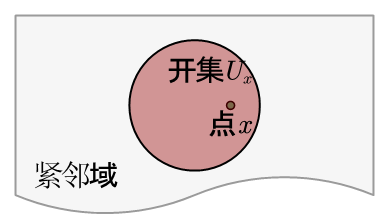
\includegraphics[width=5cm]{./figures/Topo2_1.png}
\caption{点$x$和紧邻域的关系.} \label{Topo2_fig1}
\end{figure}

紧邻域就好像是包含了$x$的一块紧子集,如果每个$x$附近都有这么一个紧子集,我们就可以在“局部”研究空间的紧性.因此我们有了以下“局部紧”的定义:

\begin{definition}{局部紧空间}
给定拓扑空间$X$和$x\in X$.如果对于某个$x\in X$及其任意邻域$U_x$,都存在一个$x$的紧邻域$C\subseteq U_x$,那么称空间$X$在$x$处\textbf{局部紧(locally compact)}.如果$X$在每一个点都局部紧,称这个空间是局部紧空间.
\end{definition}

许多紧空间之间的关系,都可以直接加上“局部”二字以后保持成立.